% !TeX root = tcolorbox.tex
% include file of tcolorbox.tex (manual of the LaTeX package tcolorbox)
% \clearpage
% Side by Side

\setcounter{section}{5}
\setcounter{subsection}{2}

\section{并排}\label{sec:sidebyside}%
\tcbset{external/prefix=external/sidebyside_}%

A \csh渐变盒子{side by side} box is a special \refEnvLe{tcolorbox} where
the upper and lower part of the box are set side by side.
All boxes of this kind are unbreakable.


一个\emph{并排}的盒子是一个特殊的\refEnvLe{tcolorbox},其中盒子的上部和下部并排设置。这种类型的所有盒子都是\csh渐变盒子[red]{不可分割的}。


\begin{marker}
% \begin{stripedbox}
Further side by side options for code examples are
% \tcblower

进一步的排版代码的 side by side 选项的例子有
% \end{stripedbox}

\refKeyLe{/tcb/listing side text},
\refKeyLe{/tcb/text side listing},
\refKeyLe{/tcb/listing outside text}, 和
\refKeyLe{/tcb/text outside listing}.
\end{marker}

% Basic Settings \hfill 
\subsection{基本设置}\label{subsec:sidebyside_basic}

% \begin{docTcbKey}{sidebyside}{=\colOpt{true\textbar false}}{默认值|true|,初始设置为|false|}
% \begin{docTcbKey}{sidebyside}{\colOpt{=true\textbar false}}{default |true|, initially |false|}
% \begin{stripedbox}
Normally, the upper part and the lower part of the box have their positions
as their names suggest. If |sidebyside| is set to |true|, the upper part
is drawn \emph{left-handed} and the lower part is drawn \emph{right-handed}.
Both parts are drawn together with the geometry settings of the upper part but the
space is divided horizontally according to the following options.
Colors, fonts, and box content additions are used individually.
The resulting box is unbreakable.

% Normally, the upper part and the lower part of the box have their positions as their names suggest. 
% 通常,盒子的upper部分和lower部分的位置,同它们的名字一致。%
% If |sidebyside| is set to |true|, the upper part
% is drawn \emph{left-handed} and the lower part is drawn \emph{right-handed}.
% 如果 |sidebyside| 设置为 true, 则upper部分会放置在左边,lower部分放置在右边。%

% Both parts are drawn together with the geometry settings of the upper part but the
% space is divided horizontally according to the following options.
% 两个部分都使用上部分的几何设置进行绘制,但空间按照以下选项水平分割。
% Colors, fonts, and box content additions are used individually.
% The resulting box is unbreakable.
% 颜色、字体和盒子内容的添加都是独立使用的。生成的盒子是\csh渐变盒子V[red]{不可分割}的。


通常,盒子的upper部分和lower部分的位置,同它们的名字一致。
如果 sidebyside 设置为 true, 则upper部分会放置在左边,lower部分放置在右边。
两个部分都使用上部分的几何设置进行绘制,但空间按照以下选项水平分割。颜色、字体和盒子内容的添加都是独立使用的。生成的盒子是\csh渐变盒子V[red]{不可分割}的。


\begin{dispExample}
\tcbset{colback=red!5!white%
,colframe=red!75!black%
,fonttitle=\bfseries}

\begin{tcolorbox}[title=我的标题,sidebyside]
这是 upper (\textit{左侧}) 部分。
\tcblower
这是 lower (\textit{右侧}) 部分。
\end{tcolorbox}
\end{dispExample}


%todo bicolor 是啥
\begin{dispExample}
% \usepackage{lipsum}
% \tcbuselibrary{skins}
\begin{tcolorbox}[bicolor% 表示创建一个双色盒子,即上下两部分的颜色可以不同。
,sidebyside%并排
,righthand width=3cm%指定右侧的宽度
,sharp corners,boxrule=.4pt,colback=green!5,colbacklower=green!50!black!50]
\lipsum[2]
\tcblower
\includegraphics[width=\linewidth]{goldshade}%
\end{tcolorbox}
\end{dispExample}
\end{docTcbKey}%
% % \clearpage
\begin{docTcbKey}[][doc updated=2015-02-06]{sidebyside align}{=\meta{alignment}}{no default, initially |center|}

Sets the vertical \meta{alignment} for the left-handed and right-handed part.%
Feasible values for \meta{alignment} are:

设置左侧和右侧的垂直 \meta{alignment} 方式。%
可选的 \meta{对齐} 值有:

\begin{tcolorbox}[title=\docValue{center},sidebyside,sidebyside align=center]
与 |minipage|环境的选项 |c| 相同。
\tcblower
identical to |minipage| option |c|.
\end{tcolorbox}
 
\begin{tcolorbox}[title=\docValue{top},sidebyside,sidebyside align=top]
与 |minipage| 选项 |t| 相同(根据基线对齐左侧和右侧的顶部行)。
\tcblower
identical to |minipage| option |t| (aligns the top lines of the left-handed and right-handed side according to their baselines).
\end{tcolorbox}

\begin{tcolorbox}[title=\docValue{bottom},sidebyside,sidebyside align=bottom]
与 |minipage| 选项 |b| 相同(根据基线对齐左侧和右侧的底部行)。
\tcblower
identical to |minipage| option |b| (aligns the bottom lines of the left-handed and right-handed side according to their baselines).
\end{tcolorbox}


\begin{tcolorbox}[title=\docValue{center seam},sidebyside,sidebyside align=center seam]
将左侧和右侧的中心对齐。
\tcblower
aligns the center of the left-handed and right-handed side.
\end{tcolorbox}

\begin{tcolorbox}[title=\docValue{top seam},sidebyside,sidebyside align=top seam]
将左侧和右侧的顶部接缝对齐。
\tcblower
aligns the very top seam of the left-handed and right-handed side.
\end{tcolorbox}


\begin{tcolorbox}[title=\docValue{bottom seam},sidebyside,sidebyside align=bottom seam]
将左侧和右侧的底部接缝对齐。
\tcblower
aligns the very bottom seam of the left-handed and right-handed side.
\end{tcolorbox}


% \begin{exdispExample}{sidebyside_align}
% \tcbset{colback=red!5!white,colframe=red!75!black,fonttitle=\bfseries,nobeforeafter,
%   left=2mm,right=2mm,sidebyside,sidebyside gap=6mm,width=(\linewidth-2mm)/3}

% \begin{tcolorbox}[adjusted title=center,sidebyside align=center]
% 这段文字太长了太长了太长了太长了,一行写不完。
% \tcblower
% 简短文字。
% \end{tcolorbox}\hfill
% \begin{tcolorbox}[adjusted title=top,sidebyside align=top]
% 这段文字太长了太长了太长了太长了,一行写不完。
% \tcblower
% 简短文字。
% \end{tcolorbox}\hfill
% \begin{tcolorbox}[adjusted title=bottom,sidebyside align=bottom]
% 这段文字太长了太长了太长了太长了,一行写不完。
% \tcblower
% 简短文字。
% \end{tcolorbox}
% \end{exdispExample}


% \begin{stripedbox}
\docValue{center}, \docValue{top}, and \docValue{bottom} are identical
to the known corresponding |minipage| options.
While this is the preferred approach for text content, the result for
boxed content like tables or images may not be as expected.
% \tcblower

\docValue{center}、\docValue{top}和\docValue{bottom}与 |minipage| 的选项相同。%
% 虽然这是文本内容的首选方法,%
% 对于盒子中是表格或图像等内容,结果可能与预期不同。
虽然这是文本内容的首选方法,但对于表格或图像等盒子内容的结果可能不如预期。
% \end{stripedbox}

% \begin{stripedbox}
For such content, one may use \docValue{center seam}, \docValue{top seam},
and \docValue{bottom seam}. For example, \docValue{top seam} aligns
the very top seam of the left-handed and right-handed side.
% \tcblower

% 对于这样的内容,可以使用\docValue{center seam}、\docValue{top seam}和\docValue{bottom seam},
% 例如,\docValue{top seam}对齐左和右边的最上面的缝。
% \end{stripedbox}

对于这样的内容,可以使用\docValue{center seam}、\docValue{top seam}和\docValue{bottom seam}。例如,\docValue{top seam}将左侧和右侧的顶部接缝对齐。


\begin{dispExample}
\tcbset{colback=red!5!white,colframe=red!75!black,fonttitle=\bfseries,
  size=small,righthand width=4cm,sidebyside,sidebyside gap=6mm,lower separated=false}

\begin{tcolorbox}[adjusted title=center seam,sidebyside align=center seam]
This is my description text for the pictures displayed on the right-handed side.
\tcblower
\includegraphics[width=\linewidth/2]{goldshade}%
\includegraphics[width=\linewidth/2]{blueshade}
\end{tcolorbox}

\begin{tcolorbox}[adjusted title=top seam,sidebyside align=top seam]
  This is my description text for the pictures displayed on the right-handed side.
  \tcblower
  \includegraphics[width=\linewidth/2]{goldshade}%
  \includegraphics[width=\linewidth/2]{blueshade}
\end{tcolorbox}

\begin{tcolorbox}[adjusted title=bottom seam,sidebyside align=bottom seam]
  This is my description text for the pictures displayed on the right-handed side.
  \tcblower
  \includegraphics[width=\linewidth/2]{goldshade}%
  \includegraphics[width=\linewidth/2]{blueshade}
\end{tcolorbox}
\end{dispExample}
\end{docTcbKey}%
% % \clearpage
\begin{docTcbKey}{sidebyside gap}{=\meta{length}}{no default, initially |10mm|}
% \begin{stripedbox}
Sets the horizontal distance between the left-handed and right-handed part to \meta{length}.
% \tcblower

将左和右部分之间的水平距离设置为\meta{length}。
% \end{stripedbox}

\begin{dispExample}
\tcbset{colback=red!5!white,colframe=red!75!black,fonttitle=\bfseries,nobeforeafter,
  sidebyside,width=(\linewidth-2mm)/2}

\begin{tcolorbox}[adjusted title=宽gap,sidebyside gap=30mm]
这段文字太长了太长了太长了太长了,一行写不完。
\tcblower
简短文字。
\end{tcolorbox}\hfill
\begin{tcolorbox}[adjusted title=窄gap,sidebyside gap=1mm]
这段文字太长了太长了太长了太长了,一行写不完。
\tcblower
简短文字
\end{tcolorbox}
\end{dispExample}
\end{docTcbKey}%
% \begin{docTcbKey}{lefthand width}{=\meta{length}}{no default, initially unset}

Sets the width of the left-handed part to the given \meta{length}.

将左部的宽度设置为给定的\meta{length}。


\begin{dispExample}
\tcbset{colback=red!5!white,colframe=red!75!black,fonttitle=\bfseries}

\begin{tcolorbox}[title=My title,sidebyside,lefthand width=3cm]
这是 upper (\textit{左}) 部分.
\tcblower
这是 lower (\textit{右}) 部分.
\end{tcolorbox}
\end{dispExample}
\end{docTcbKey}

\enlargethispage*{1cm}
\begin{docTcbKey}{righthand width}{=\meta{length}}{no default, initially unset}

Sets the width of the right-handed part to the given \meta{length}.

将右部的宽度设置为给定的\meta{length}。


\begin{dispExample}
\tcbset{colback=red!5!white,colframe=red!75!black,fonttitle=\bfseries}

\begin{tcolorbox}[title=My title,sidebyside,righthand width=3cm]
这是 upper (\textit{左}) 部分.
\tcblower
这是 lower (\textit{右}) 部分.
\end{tcolorbox}
\end{dispExample}
\end{docTcbKey}

% \clearpage
\begin{docTcbKey}{lefthand ratio}{=\meta{fraction}}{no default, initially |0.5|}

Sets the width of the left-handed part to the given \meta{fraction} of
the available space. \meta{fraction} is a value between |0| and |1|.

设置左侧的宽度为所有可用宽度的比例 \meta{fraction}。
\meta{fraction} 取值在 |0| 到 |1|。


\begin{dispExample}
\tcbset{colback=red!5!white,colframe=red!75!black,fonttitle=\bfseries}

\begin{tcolorbox}[title=My title,sidebyside,lefthand ratio=0.25]
这是 upper (\textit{左}) 部分.
\tcblower
这是 lower (\textit{右}) 部分.
\end{tcolorbox}
\end{dispExample}
\end{docTcbKey}


\begin{docTcbKey}{righthand ratio}{=\meta{fraction}}{no default, initially |0.5|}

Sets the width of the right-handed part to the given \meta{fraction} of
the available space. \meta{fraction} is a value between |0| and |1|.

设置右侧的宽度为所有可用宽度的比例 \meta{fraction}。
\meta{fraction} 取值在 |0| 到 |1|。


\begin{dispExample}
\tcbset{colback=red!5!white,colframe=red!75!black,fonttitle=\bfseries}
\begin{tcolorbox}[title=My title,sidebyside,righthand ratio=0.25]
这是 upper (\textit{左}) 部分.
\tcblower
这是 lower (\textit{右}) 部分.
\end{tcolorbox}
\end{dispExample}
\end{docTcbKey}


% \clearpage

If one side of a side-by-side box should be adapted to the width of its content, 
this width has to be computed beforehand.
The following example uses a savebox |\mysavebox| to store the picture to determine its width. 
A more convenient way to handle this task is to use the methods from \Fullref{subsec:sidebyside_xparse}.

如果一个并排的盒子的一边要适应其内容的宽度, %
这个宽度必须事先计算。%
下面的例子使用一个存储盒子 |\mysavebox| 来存储图片以确定其宽度。%
处理这个任务更方便的方法是使用来自 \Fullref{subsec:sidebyside_xparse} 的方法。

\begin{引述之言}{virhuiai}
可以在code中处理,见下面的例子。
\end{引述之言}
% code={\sbox{\mysavebox}{#2}},
% lefthand width=\wd\mysavebox,

\begin{dispExample}
% \tcbuselibrary{skins,xparse}
% \usepackage{lipsum}
% \newsavebox\mysavebox  % preamble
\DeclareTotalTColorBox{\mysidebox}{ O{} +m +m }{
  bicolor,colback=white,colbacklower=yellow!10,
  fonttitle=\bfseries,center title,
  sidebyside,
  code={\sbox{\mysavebox}{#2}},
  lefthand width=\wd\mysavebox,
  drop lifted shadow,
  #1
}
{\usebox{\mysavebox}\tcblower#3}

\mysidebox[title=The Triangle]{%
  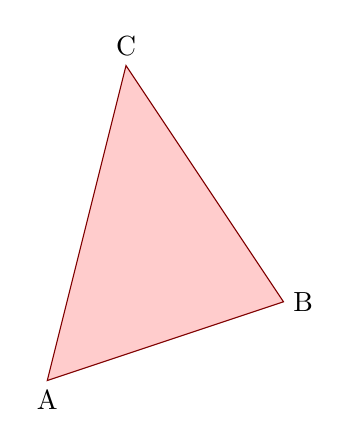
\begin{tikzpicture}
    \path[fill=red!20,draw=red!50!black]
      (0,0) node[below]{A} -- (3,1) node[right]{B}
      -- (1,4) node[above]{C} -- cycle;
  \end{tikzpicture}%
}{%
  \lipsum[1]
} 
\end{dispExample}% % code={\sbox{\mysavebox}{#2}}, % lefthand width=\wd\mysavebox, 学习了


 
\end{document}




% \clearpage
% Advanced Settings from the \mylib{xparse} Library
\subsection{来自\mylib{xparse}库的高级设置}\label{subsec:sidebyside_xparse}

\begin{marker}
\begin{stripedbox}
All following macros and options need the \mylib{xparse} library to be
loaded, see \Fullref{sec:xparse}.
\tcblower
所有下面的宏和选项都需要加载 \mylib{xparse}库,见\Fullref{sec:xparse}。
\end{stripedbox}
\end{marker}


\begin{docCommand}[doc new=2015-11-20]{tcbsidebyside}{\oarg{options}\marg{left-handed content}\marg{right-handed content}}
\begin{stripedbox}
Creates a colored box using more or less arbitrary \meta{options} for a \refEnvLe{tcolorbox}.
The \refKeyLe{/tcb/sidebyside} option is set to |true| and the \meta{left-handed content} and \meta{right-handed content} is filled into the box appropriately.
The resulting box is unbreakable.
\tcblower
为\refEnvLe{tcolorbox}指定任意的选项\meta{options}创建一个 |tcolorbox| 盒子。%
\refKeyLe{/tcb/sidebyside}选项被设置为|true|, \meta{left-handed content}和\meta{right-handed content}被适当地填充到盒子中。%
这样的盒子是不可分页的。
\end{stripedbox}

\begin{stripedbox}
\refComLe{tcbsidebyside} is not only a shortcut for using a normal \refEnvLe{tcolorbox} with \refKeyLe{/tcb/sidebyside}, 
but allows setting further options like \refKeyLe{/tcb/sidebyside adapt} and \refKeyLe{/tcb/sidebyside switch}.
\tcblower
\refComLe{tcbsidebyside}不只是使用普通的\refEnvLe{tcolorbox}指定\refKeyLe{/tcb/sidebyside}的快捷方式, 
还允许设置更多的选项,如\refKeyLe{/tcb/sidebyside adapt}和\refKeyLe{/tcb/sidebyside switch}。
\end{stripedbox}

\begin{dispExample}
% \tcbuselibrary{skins,xparse}
% \usepackage{lipsum}
\tcbsidebyside[title=The Triangle,
  sidebyside adapt=left,
  bicolor,colback=white,colbacklower=yellow!10,
  fonttitle=\bfseries,center title,drop lifted shadow,
]{%
  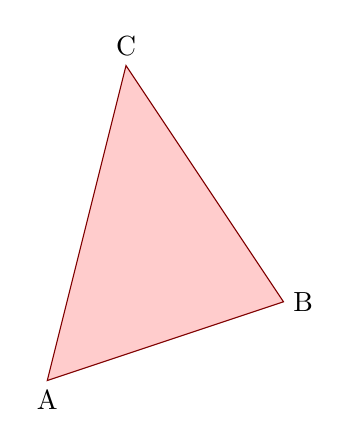
\begin{tikzpicture}
    \path[fill=red!20,draw=red!50!black]
      (0,0) node[below]{A} -- (3,1) node[right]{B}
      -- (1,4) node[above]{C} -- cycle;
  \end{tikzpicture}%
}{%
  \lipsum[1]
}
\end{dispExample}
\end{docCommand}

% \clearpage
\begin{docTcbKey}[][doc new=2015-11-20]{sidebyside adapt}{=\meta{side(s)}}{no default, initially |none|}
\begin{stripedbox}
The option allows the left-handed and/or right-handed side to determine the dimensions of the box. 
This option is only valid inside \refComLe{tcbsidebyside}.
\tcblower
该选项允许根据左边和/右边内容确定盒子的尺寸。
此选项仅在\refComLe{tcbsidebyside}内有效。
\end{stripedbox}

Feasible values for \meta{side(s)} are:
\begin{itemize}
    \item\docValue{none}: 
\begin{stripedbox}
no measurement of left-handed and right-handed side.
\tcblower
不测量左边和右边。
\end{stripedbox}
    \item\docValue{left}:
\begin{stripedbox}
the actual width of the left-handed content is used to set \refKeyLe{/tcb/lefthand width}.
\tcblower
左侧内容的实际宽度用于设置 \refKeyLe{/tcb/lefthand width}。
\end{stripedbox}
    \item\docValue{right}:
\begin{stripedbox}
the actual width of the right-handed content is used to set \refKeyLe{/tcb/righthand width}.
\tcblower
右侧内容的实际宽度用于设置\refKeyLe{/tcb/右手宽度}。
\end{stripedbox}

    \item\docValue{both}:
\begin{stripedbox}
the actual width of the left-handed and right-handed content is used to set \refKeyLe{/tcb/lefthand width},  \refKeyLe{/tcb/righthand width}, and the overall \refKeyLe{/tcb/width}.
\tcblower
左手和右手内容的实际宽度用于设置 \refKeyLe{/tcb/lefthand width} 和 \refKeyLe{/tcb/righthand width},%
和整个\refKeyLe{/tcb/width}。
\end{stripedbox}

\end{itemize}

\begin{dispExample}
% \tcbuselibrary{skins,xparse}
\tcbsidebyside[sidebyside adapt=left,
  title=非常重要的表格,
  beamer,colframe=blue!50!black,colback=blue!10
  ,lower separated=false%无分隔线了
  ,sidebyside gap=5mm
]{%
  \begin{tabular}{|l|c|r|}\hline
    left & center & right\\\hline
    A & B & C\\\hline
    D & E & F\\\hline
  \end{tabular}
}{%
此表包含所有未来操作的最重要数据。
你可能注意到B跟在A后面,C跟在B后面,以此类推。
}
\end{dispExample}



\begin{dispExample}
% \tcbuselibrary{skins,xparse}
\tcbsidebyside[sidebyside adapt=right,
  blanker,sidebyside gap=5mm
]{%
  \lipsum[2]
}{%

\begin{tikzpicture}
  \path[fill=yellow,draw=yellow!75!red] (0,0) circle (1cm);
  \fill[red] (45:5mm) circle (1mm);
  \fill[red] (135:5mm) circle (1mm);
  \draw[line width=1mm,red] (215:5mm) arc (215:325:5mm);
\end{tikzpicture}
}
\end{dispExample}


\begin{dispExample}
% \tcbuselibrary{skins,xparse}
\tcbsidebyside[sidebyside adapt=both,
  enhanced,center,
  title=Both sides adapted,
  attach boxed title to top center={yshift=-2mm},
  coltitle=black,boxed title style={colback=red!25},
  segmentation style=solid,colback=red!5,colframe=red!50
]{%
  \begin{tabular}{|l|c|r|}\hline
    left & center & right\\\hline
    A & B & C\\\hline
    D & E & F\\\hline
  \end{tabular}
}{%

\begin{tikzpicture}
  \path[fill=yellow,draw=yellow!75!red] (0,0) circle (1cm);
  \fill[red] (45:5mm) circle (1mm);
  \fill[red] (135:5mm) circle (1mm);
  \draw[line width=1mm,red] (215:5mm) arc (215:325:5mm);
\end{tikzpicture}
}
\end{dispExample}
\end{docTcbKey}

% \clearpage
\begin{docTcbKey}[][doc new=2015-11-20]{sidebyside switch}{\colOpt{=true\textbar false}}{default |true|, initially |false|}
\begin{stripedbox}
If set to |true|, the
\meta{left-handed content} and \meta{right-handed content}
of \refComLe{tcbsidebyside} are switched.
Obviously, this option is only valid inside \refComLe{tcbsidebyside}.
\tcblower
如果设置为|true|,%
\refComLe{tcbsidebyside}的 \meta{left-handed content} 和 \meta{right-handed content} 会被切换。%
显然,这个选项只在\refComLe{tcbsidebyside}内有效。
\end{stripedbox}

\begin{stripedbox}
The side switching can be made even/odd page sensitive, 
if used inside \refKeyLe{/tcb/if odd page}.
\tcblower
如果指定了了 \refKeyLe{/tcb/if odd page},两侧切换对奇/偶页敏感。
\end{stripedbox}


\begin{dispExample}
% \tcbuselibrary{skins,xparse}
\tcbsidebyside{Left}{Right}

\tcbsidebyside[sidebyside switch]{Left}{Right}

\tcbsidebyside[title=Very important table,
  if odd page={sidebyside switch,sidebyside adapt=right,flushright title}%
              {sidebyside adapt=left},
  beamer,colframe=blue!50!black,colback=blue!10,
  lower separated=false,sidebyside gap=5mm
]{%
  \begin{tabular}{|l|c|r|}\hline
    left & center & right\\\hline
    A & B & C\\\hline
    D & E & F\\\hline
  \end{tabular}
}{%
  This table contains the most important figures for
  all future actions. You may notice that B follows A,
  C follows B, and so on.
}
\end{dispExample}


\end{docTcbKey}

